\documentclass{article} % For LaTeX2e
\usepackage{nips13submit_e,times}
\usepackage{graphicx}
\usepackage{hyperref}
\usepackage{amsmath}
\usepackage{subcaption}
\usepackage{amssymb}
\usepackage{algorithm}
\usepackage{algpseudocode}
\usepackage{url}
\usepackage[
abbreviate=false,
backend=biber,
sortcites=true,
sorting=nyt,
sortlocale=en_US,
style=numeric-verb,
maxnames=10
]{biblatex}                     % Bibliography support

\newcommand{\setof}[1]{\ensuremath{\left \{ #1 \right \}}}

\title{Multi-armed Bandits and Reinforcement Learning Approaches to Targeted
Advertising}


\author{
Eric Andrews \\
Seminar: Reinforcement Learning and Its Applications, Spring 2014 \\
Department of Computer Science, University of Helsinki\\\\
}

% The \author macro works with any number of authors. There are two commands
% used to separate the names and addresses of multiple authors: \And and \AND.
%
% Using \And between authors leaves it to \LaTeX{} to determine where to break
% the lines. Using \AND forces a linebreak at that point. So, if \LaTeX{}
% puts 3 of 4 authors names on the first line, and the last on the second
% line, try using \AND instead of \And before the third author name.

\newcommand{\fix}{\marginpar{FIX}}
\newcommand{\new}{\marginpar{NEW}}


\nipsfinalcopy % Uncomment for camera-ready version

\bibliography{sources.bib}
\begin{document}


\maketitle

\begin{abstract}
  On the Internet, content producers often rely on profits made through banner
  ad clicks. Thus it is of interest to find ways to increase banner ad
  click-through rates (CTR). One way to further this goal is targeted
  advertising, in which the profile of the visiting user is used to determine
  which ads he or she would be interested in. This seminar report surveys
  multi-armed bandit and reinforcement learning approaches to targeted
  advertising. Thompson sampling, mortal bandits, as well as temporal
  difference learning are the methods considered.
\end{abstract}

\section{Introduction}

In an age where a huge amount of information and news can be found
free-of-charge online, many content producers on the Internet rely on
advertisement revenues to fund their operations. Often this advertisement is
deployed in the form of clickable banner ads, either textual, graphical,
animated or even interactive content, usually separated from the main content,
and designed to attract the interest of visitors. When a visitor clicks such a
banner, they are redirected to the advertiser's site, and the content producer
is financially compensated for the referral.

In this kind of advertising, it is the interest of the content producer to
maximize \emph{click-through rate} (CTR) of the banner ads: the number of times
clicked divided by \emph{impressions}, the number of times shown. If a content
producer has several ad banners it could show to the user, one strategy could
be just to fill up the web site with ads. However this can quickly lead to user
annoyance, and in the worst scenario, cause users to leave the site. Further,
the effectiveness of the advertisements starts to wither as more slots for
banners are introduced, either because a saturation point is hit where users
learn to ignore most of the banners, or there simply is not room for more
banners on the page.

An alternative strategy is to recognize that there is a limit to the number of
viable banner slots, and attempt to somehow selectively choose the ads to show
according to whom the ad is being displayed to. This is often referred to as
\emph{targeted advertising} or \emph{behavioral targeting}. By adding some
intelligence, we can attempt to show the user advertisements he or she could
potentially be interested in instead of just uniformly picking one out of a
bunch.

This paper introduces two approaches to targeted advertising. First the
simpler, multi-armed bandit model is explored in some detail. It is the classic
example through which the exploration vs.  exploitation trade-off has been
studied. We then delve into some modifications of the model that are useful in
this setting of banner ad selection. After going through this simple model, a
more complex approach called reinforcement learning is considered. This
approach allows us to take into consideration situations in which the agent,
the ad system, can affect the state of the user, e.g. make them annoyed so that
they leave the site.

\section{Related work}

Other approaches to targeted advertising have been explored as well. Chen et
al. \cite{chen2009large} consider a Poisson regression model to predict
click-through rates from user history.  They applied their large-scale
parallelized approach to Yahoo's user base which resulted in great improvement
in CTR.

Work in information retrieval may be applied to targeted advertising as well.
For example personalized news recommendation is in some sense a very similar
problem, albeit from a different viewpoint. \emph{Contextual advertising} is
also concerned with selecting banner ads intelligently, but instead of
targeting the user, the ad is chosen according to the content being served to
the user.

A different but domain-related topic is learning strategies for
\emph{real-time bidding}. Currently web sites can sell ads for banner slots at
an extremely granular level: a single impression. When a user visits a site, a
few hundred millisecond auction is held, in which the advertisers name their
price given the profile of the visiting user. When the time is up, the highest
bidder gets their ad on the site. There have been studies on optimal strategies
for maximizing profits (i.e. balancing ad click-rate and cost) from the
viewpoint of the advertiser with \cite{ding2013multi} and without
\cite{chakraborty2010selective} the multi-armed bandit model. In any case, the
exploration vs exploitation dilemma is highlighted in this setting.

The quite recent field of applying computer science to ad selection goes under
the umbrella term \emph{computational advertising}. Especially software
corporations Microsoft and Yahoo conduct applied research in this field, while
the National Institute of Statistical Science (NISS) held a workshop on the
topic in 2009. % wikipedia

\section{Approaches}

Depending upon what kind of aspects of the problem we wish to take into
consideration, we may either consider targeted advertising through the simpler
bandit approach, or, the more complex full reinforcement learning approach. The
first approach is limited to immediate rewards while the second can learn from
delayed rewards, i.e. rewards that are not necessarily received immediately
after performing an action \cite{silver2013concurrent}. The reinforcement
learning approach can also capture effects the ad displayer (the agent) has
on the user (the state), for example user attrition caused by an offensive ad.

% Why important the above?


\subsection{Contextual bandit}

In the standard $n$-armed bandit problem, we are facing a slot machine with $n$
levers. Each lever is associated with some distinct probability distribution
that determines the amount of reward received from pulling that lever. Assuming
that pulling a lever is free, but that we have a limited number of pulls, how
do we maximize the expected total reward given that we do not know the
underlying distributions? \cite{book}

In the above situation, the \emph{exploration vs. exploitation} dilemma is
highlighted. After playing for a bit, we may get a sense that some lever has
rewarded us better than the rest based on our experience so far. Do we, then,
greedily continue playing that arm till the end, \emph{exploiting} our current
knowledge? Or should we still \emph{explore} the other levers, in case we have
had bad luck and another lever has better payout in the long run? These are the
questions that bandit algorithms attempt to answer in an optimal way.

We are especially interested in a generalization of the $n$-armed bandit
problem, namely the \emph{contextual multi-armed bandit}
\cite{langford2007epoch}, in which we receive some side-information, a context,
before having to choose the lever to pull. The setting has been outlined below.

\begin{itemize}
  \item[]
    \textbf{For} $t = 1, ..., T$ (rounds)
    \begin{enumerate}
      \item{Receive some context $x_t$.}
      \item{Choose action  $a_i$ (pull lever), where $i \in \setof{1,...,n}$.}
      \item{Receive reward $r_t \in \mathbb{R}$.}
    \end{enumerate}
\end{itemize}

It should be stated that even though at first glance the multi-armed bandit
may seem like a very contrived problem, it is actually a very general
framework. In the case of targeted advertising, one way to adapt this model
is as follows.  The agent making the decisions is the website. The levers to
pull are all the possible ads that can be shown in a banner slot. The reward
received is 1 if a user clicks the ad, and 0 otherwise. The context is some
information gathered on the user, e.g. what pages they have visited, gender,
interests, age and so on. A more complex reward function could also be
considered, in which the reward received depends, for example, on which ad is
being displayed.

\subsubsection{Thompson sampling}
Thompson sampling \cite{chapelle2011empirical} is an algorithm to address the
exploitation vs. exploration trade-off in the contextual multi-armed bandit
case. The idea is that we have a probability distribution on the arms denoting
the probability that each is optimal. In each round, we sample these
distributions so as to choose the next lever to pull. The distributions are
then updated according to rewards experienced.

Thompson sampling can be understood in the Bayesian context as follows. Denote
previous observations of contexts, pulls and rewards as $D = \setof{(x_i, a_i,
r_i) \;|\; i \in \mathbb{N}}$. These are modeled using a likelihood function
$P(r \;|\; a,x,\theta)$, where $\theta$ are some parameters. The posterior
distribution of the parameters is given by the Bayes rule, namely $P(\theta |
D) \propto \prod P(r_i | a_i, x_i, \theta) P(\theta)$, given prior $P(\theta)$.

Assuming we knew the true parameters $\theta^*$, we would ideally choose the
lever that maximizes expected reward $\arg\max_a E[r | a, x, \theta^*]$. In
reality we do not know the true parameters. Instead, we must integrate over the
domain of the parameters $\theta$, obtaining $\arg\max_a \int E[r | a, x,
\theta] P(\theta|D) d\theta$. However this corresponds to only exploitation
\cite{chapelle2011empirical}.

Taking exploration into consideration as well, the following equation is
obtained: the probability of choosing to perform pull $a$ is given by
\begin{equation}
  \int \mathbb{I}\bigg[E[r|a,x,\theta] = \max_{a'}
  E\big[r|a',x,\theta\big]\bigg] P(\theta | D) d\theta,
\end{equation}

where $\mathbb{I}$ is an indicator function that obtains value 1 when its
condition is true and zero when it is not.  This integral is not directly
computed, instead Algorithm~\ref{alg:thompson} is used to the same effect.

\begin{algorithm}
  \caption{Thompson sampling \cite{chapelle2011empirical}}
  \label{alg:thompson}
  \begin{algorithmic}[1]
    \State $D := \emptyset$
    \For{$t=1,...,T$}
      \State Receive context $x_t$.
      \State Draw $\theta^t$ according to $P(\theta | D)$.
      \State Select $a_t := \arg\max_a E[r | x_t, a, \theta^t]$.
      \State Observe reward $r_t$.
      \State $D = D \cup (x_t, a_t, r_t)$.
    \EndFor
  \end{algorithmic}
\end{algorithm}

Let us illustrate this idea with the help of an example. Assume the standard
$n$-armed bandits situation, in which each lever $i \in [1,n]$ is distributed
according to a Bernoulli distribution with success probability $\theta^*_i$.
This is equivalent to a biased coin flip, in which heads ($r=1$) is observed
with probability $\theta^*_i$ and tails ($r=0$) with probability $1 -
\theta^*_i$.

For each arm $i$, we maintain a separate Beta distribution modeling our belief
of what the arm's success probability (or CTR) is. In mathematical terms, if
$X_i$ is the random variable corresponding to the reward received (coin flip,
click or not, 0 or 1) from pulling the $i$:th lever, then $X_i \sim
\text{Bernoulli}(\theta^*_i)$, and we estimate $E[X_i] \sim \text{Beta}(S_i +
1, F_i + 1)$, where $S_i$ is the number of successes and $F_i$ is the number of
failures observed for the $i$:th arm so far. The Beta distribution is used
because it is the conjugate prior of the Bernoulli likelihood, a concept from
Bayesian probability theory that roughly states that the posterior distribution
stays in the same family as the prior distribution. Furthermore, the math works
out in an intuitive sense.

This example is applied as Algorithm~\ref{alg:thompson} as follows. We
initialize $S_i := F_i := 0$ for all arms. Line 3 can be ignored because we are
not considering context. Line 4 is performed so that each arm's Beta
distribution is sampled.  The arm with the largest sample is pulled, and its
respective success or failure counter is updated after receiving the reward.
This is equivalent to the posterior update on Line 7.  The pseudocode for this
Bernoulli case has been outlined in Algorithm~\ref{alg:thompson-bandit}.

\begin{algorithm}[H]
  \caption{Thompson sampling for the Bernoulli bandit, adapted from \cite{chapelle2011empirical}}
  \label{alg:thompson-bandit}
  \begin{algorithmic}[1]
    \Require Prior parameters $\alpha$ and $\beta$ of a Beta distribution.
    Typical value is 1.
    \State $S_i := F_i := 0, \; \forall i \in [1,K]$.
    \For{$t=1,...,T$ (each round)}
      \For{$k=1,...,K$ (each arm)}
      \State Draw $\theta_i \sim \text{Beta}(S_i + \alpha, F_i + \beta)$
      (sample each arm).
      \EndFor
      \State Draw arm $\hat{i} := \arg\max_{i} \theta_i$ (with largest sample) and observe reward $r$.
      \If {$r=1$}
      \State Increment success counter $S_{\hat{i}} := S_{\hat{i}} + 1$.
      \Else
        \State Increment failure counter $F_{\hat{i}} := F_{\hat{i}} + 1$.
      \EndIf
    \EndFor
  \end{algorithmic}
\end{algorithm}

How a Beta distribution, conveying our belief on click probability for an arm,
can look like, is illustrated in Figure~\ref{fig:beta}. Shown is the history of
a Beta distribution for a single arm. Naturally, each arm would have a history
of Beta distributions running parellel to the one shown in
Figure~\ref{fig:beta}.

From left to right of Figure~\ref{fig:beta}, we start off with the initial
situation in which no observations have yet been done. The uniform prior,
$\alpha = \beta = 1$, is used so that each success probability $\theta^*_i$ is
believed to be equally likely.

The second plot shows how the distribution looks like after we have observed
one click of the respective ad. Our beliefs shift towards higher click-through
rates. In the third plot, 6 clicks and 3 non-clicks have been recorded.
Non-clicks cause the distribution to shift a bit leftwards towards lower CTR.
The final figure shows how the distributions looks like after 300 clicks and 60
non-clicks. We see how the distribution sharpens --- it is more confident that
the 'true' CTR lays at about $300 / 360 \approx 0.833$.

\begin{figure}[H]
  \centering
  \begin{subfigure}{.25\textwidth}
    \centering
    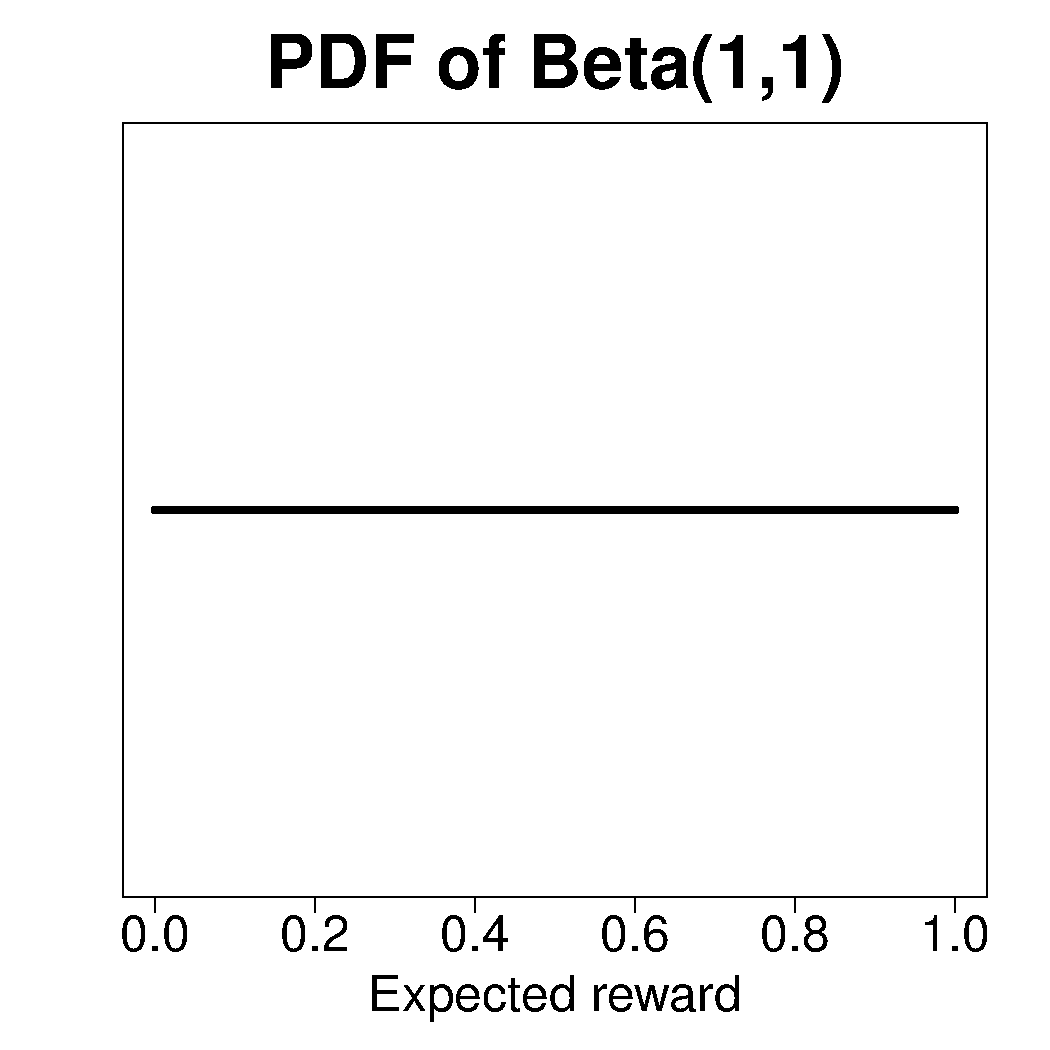
\includegraphics[width=.9\linewidth]{beta1.pdf}
  \end{subfigure}%
  \begin{subfigure}{.25\textwidth}
    \centering
    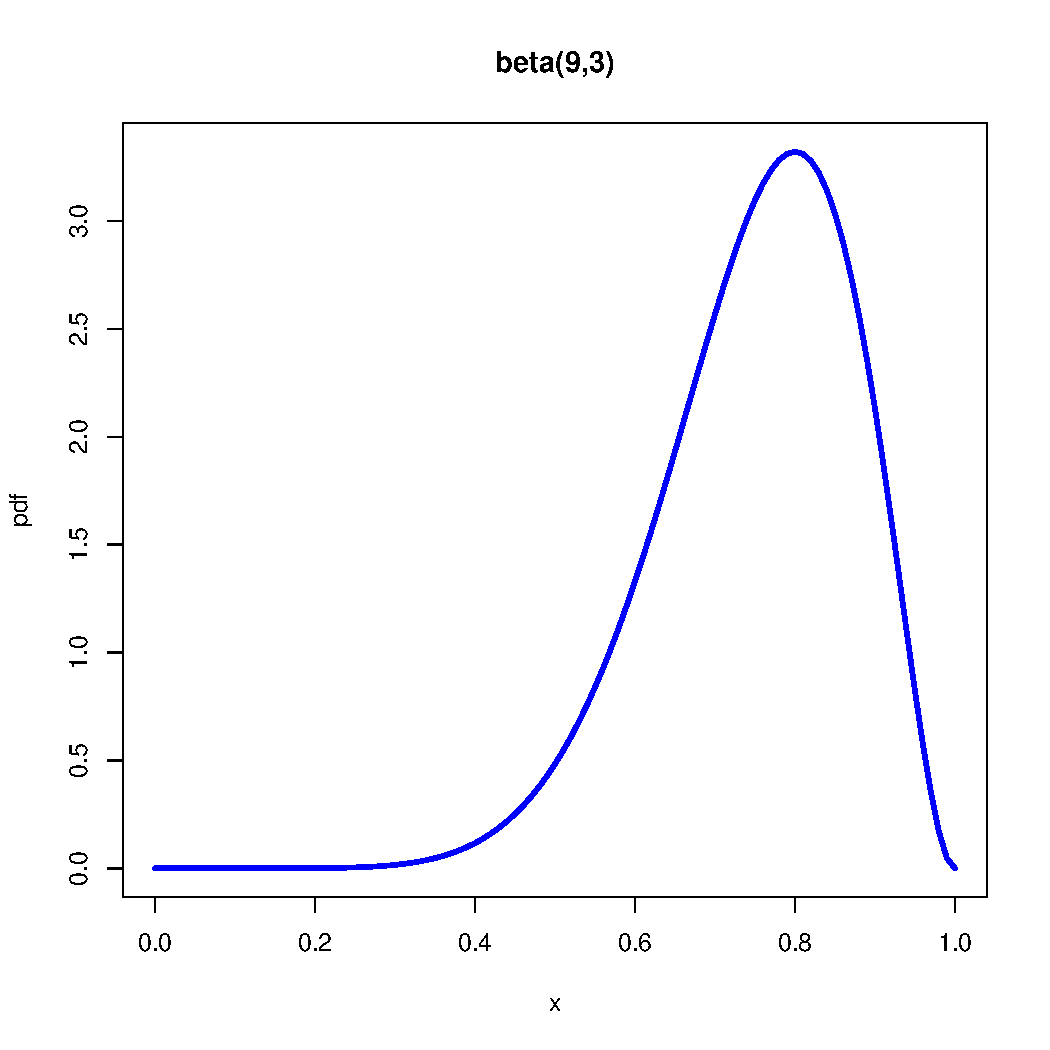
\includegraphics[width=.9\linewidth]{beta2.pdf}
  \end{subfigure}%
  \begin{subfigure}{.25\textwidth}
    \centering
    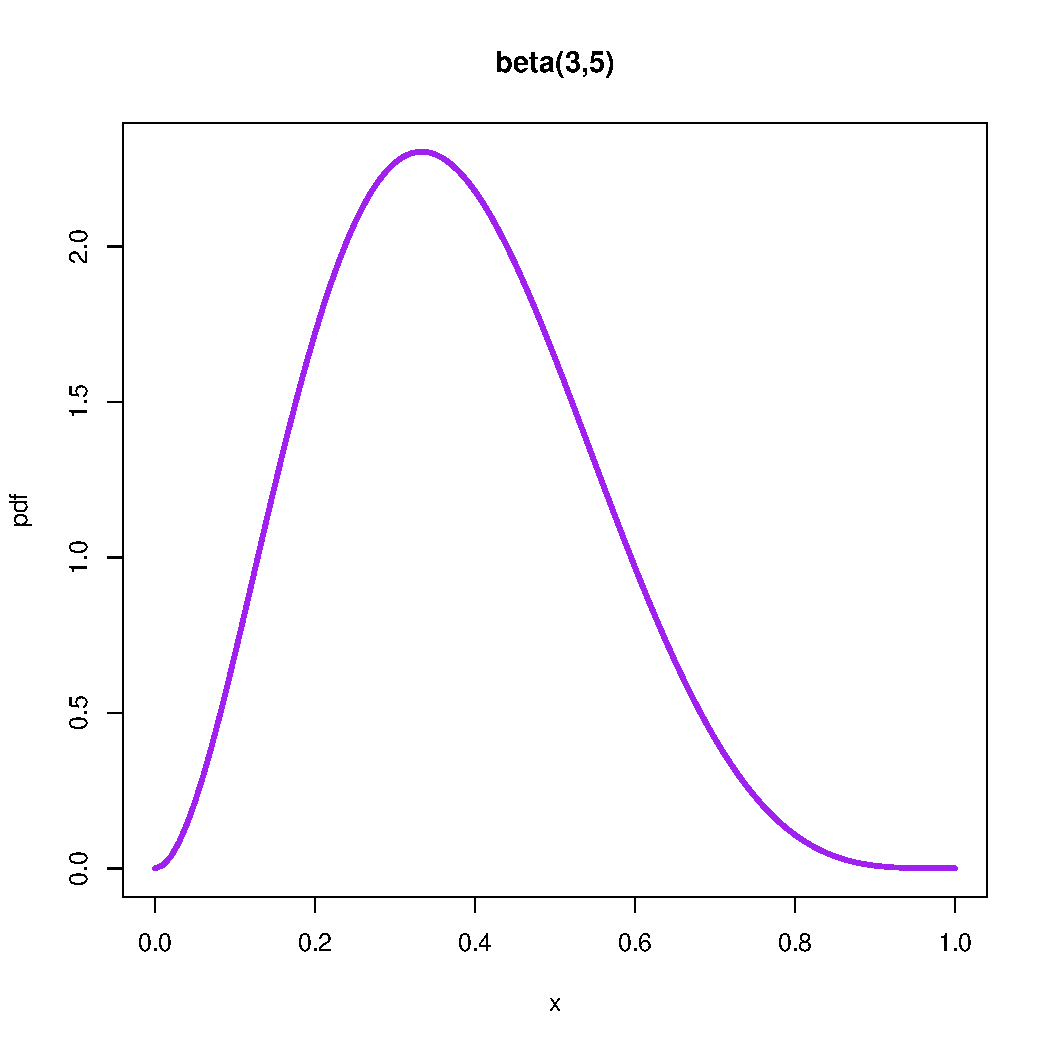
\includegraphics[width=.9\linewidth]{beta3.pdf}
  \end{subfigure}%
  \begin{subfigure}{.25\textwidth}
    \centering
    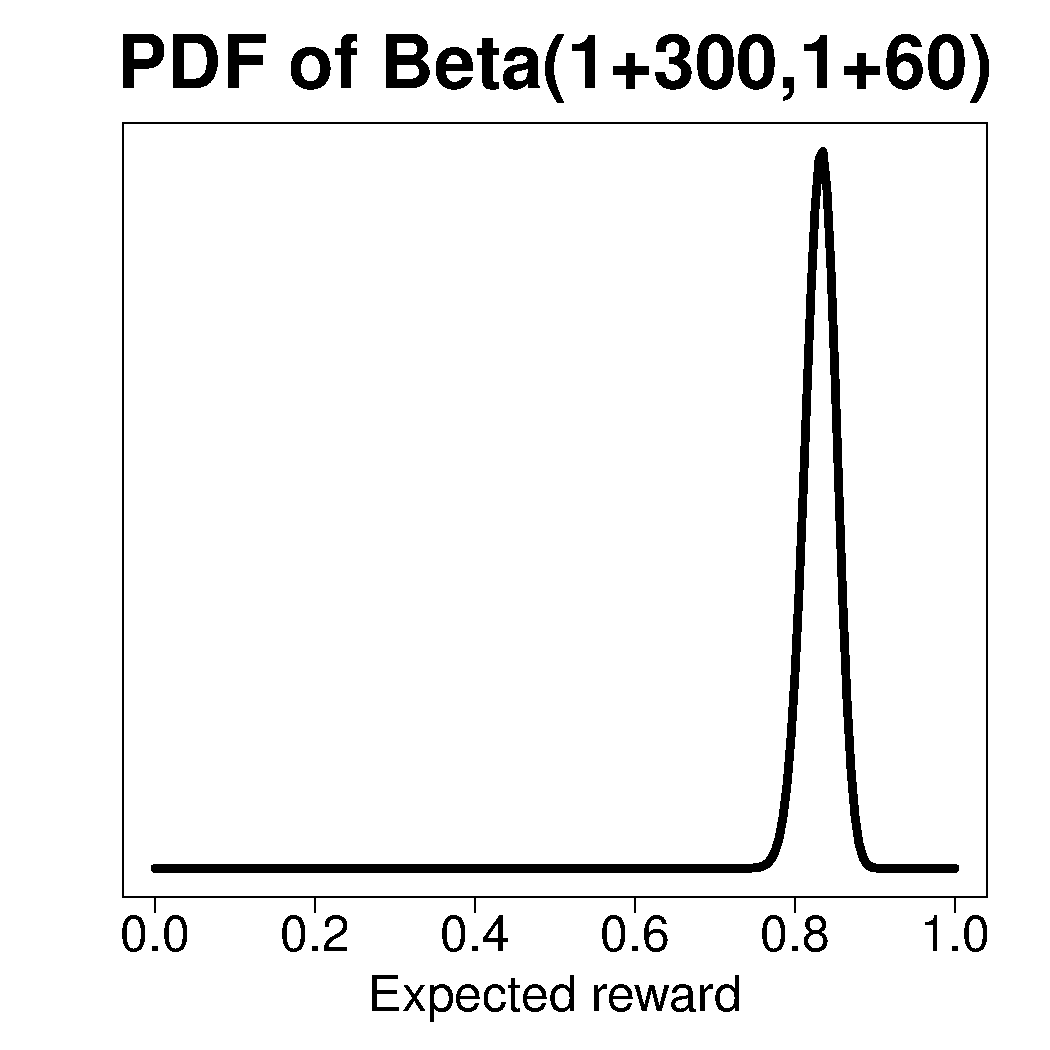
\includegraphics[width=.9\linewidth]{beta4.pdf}
  \end{subfigure}
  \caption{Illustration on what a series of Beta distributions modeling the
  success probability of a Bernoulli distribution can look like. On the very
left is the initial uniform situation when nothing has yet been observed. Then
a single ad click click ($r=1$) is observed, which tilts our belief to higher click
rates. Then 5 clicks ($r=1$, successes) and 2 non-clicks ($r=0$, failures) are
recorded. The final situation to the very right shows what the distribution
looks like after 300 clicks and 60 non-clicks.}
  \label{fig:beta}
\end{figure}

Figure~\ref{fig:beta} highlights the situation for only a single arm (ad).
Each ad will have a respective series of Beta distributions according to
history of clicks observed. At round $t$ we sample each ad's current
distribution, as in Lines 3-5 of Algorithm~\ref{alg:thompson-bandit}, and show
the ad with the highest sample. This means that in the long run, when the
distributions settle on some peaks, the algorithm will start to exploit.
However there is still randomness involved, and occasionally, other ads will be
shown as well, and their respective distributions updated.

The parameters to tinker with in this situation are the priors $\alpha$ and
$\beta$. They can be set uniquely for each distribution to model our prior
belief that some ads will be clicked on more than others, if, we have a strong
conviction that such is the case. Chapelle et al. \cite{chapelle2011empirical}
note that even with prior mismatches, Thompson sampling works well. Thus the
defaults are often good enough in practice.

We can also reshape the posterior distributions to be more sharp, thereby
favoring exploitation, or, we can widen them to favor exploration. The latter
may be useful in situations where the distributions are highly nonstationary.
For example, in the ad banner domain, it may be that users get tired of the
same ads being displayed over a long period of time. Perhaps some big news
event happens and suddenly users are interested in clicking an ad that used to
be uninteresting to them. Hence estimated sharp click-through rates are no
longer acccurate, and more uncertainty should be introduced in the form of
widening the posteriors.

In the example above, we did not consider context.  To use contexts in this
Thompson setting, we need a separate distribution for each ad and user profile
pair. Not surprisingly then, if the number of ads, and especially, if the
number of possible user profiles is too high, we need a huge set (possibly of
infinite cardinality) of distributions. What follows easily is that we
encounter a situation, where there are too many parameters to learn reliably.
There are ways to combat this as will be seen in
Section~\ref{sec:function_approximation}.

While the presented approach is Bayesian, it is not fully Bayesian like the
Gittins index, which although is Bayes-optimal, can not be implemented
efficiently in practice \cite{chapelle2011empirical}. The downside of Thompson
sampling is that there is a lack of theoretical analysis. Chapelle et al.
\cite{chapelle2011empirical}, however, demonstrate empirically that it
outperforms UCB \cite{auer2002finite} and $\epsilon$-greedy methods in certain
cases.

One such case is delayed feedback which is central to ad display. We may
not process the rewards immediately because of runtime or user constraints,
e.g. system is not fast enough or user does not immediately click on ad when on
page. The feedback might be processes in batches between which lay a long
amount of time. Thompson sampling alleviates the problem of delayed feedback by
randomization over actions, while deterministic UCB suffers large regret when
it gets locked on to a suboptimal choice.

\subsubsection{Mortal bandits}
Most often in online advertisement, the ads (the levers) have a limited
lifespans due to limited budgets, seasonal holiday campaigns, and other
uncontrollable factors. On the other hand, new levers are introduced
occasionally in the form of new ad campaigns. This results in a stark
contradiction between reality and our model, because the multi-armed bandit
model assumes implicitly that its levers are in existence indefinitely
\cite{chakrabarti2008mortal}.

Chakrabarti et al. \cite{chakrabarti2008mortal} introduce algorithms for mortal
multi-armed bandits, a model in which levers regularly die and new ones come to
existence as replacements. One of the main results they derive is that the
regret bounds for such a situation can not be as low as for the non-mortal
case. Instead of $O(\ln t)$, a bound of $\Omega(t)$ is achieved under
mortality, $t$ being the number of rounds.

One of the main reasons for the worse bound is that in the non-mortal scenario,
after finding an optimal arm, the algorithm can thereafter concentrate on
indefinite exploitation. (Maybe doing some exploration on the side as well, to
account for nonstationarity.) When arms are subject to lifetimes, such
nonchalance is out of the question.  An especially challenging case arises when
there are many levers and short lifespans. Most likely, one must settle for
suboptimality in such a case.

The paper \cite{chakrabarti2008mortal} also describes how standard multi-armed
bandits can be adapted to take mortality into account. This is needed so that
the algorithms do not spend too much time on exploration, an investment that is
not justified under mortality. The idea of the \emph{subset heuristic} is to
divide the rounds $t=1...T$ into epochs. At the dawn of each epoch, we choose a
subset of arms uniformly at random from the set of all arms. We then run the
standard multi-armed bandit algorithm on the subset until the end of the epoch.
This method is outlined in Algorithm~\ref{alg:subsetheuristic}.

\begin{algorithm}
  \caption{Subset heuristic, adapted from \cite{chakrabarti2008mortal}}
  \label{alg:subsetheuristic}
  \begin{algorithmic}[1]
    \Require Integer $c \in [1,K]$, any standard multi-armed bandit algorithm
    $A$
    \For{$t=1,...,T$ (each round)}
      \State $S := $ choose $K/c$ random arms.
      \State $dead := 0$.
      \State Initialize algorithm $A$ over arms $S$.
      \Repeat
        \State Select arm $i$ using algorithm $A$.
        \State Pull arm $i$, provide reward to $A$.
        \State $S_d :=$ arms that died during turn.
        \State $S := S \setminus S_d$
        \State $dead := dead + |S_d|$.
      \Until{$dead \geq K/2$ \textbf{or} $|S| = 0$}
    \EndFor
  \end{algorithmic}
\end{algorithm}

Let us summarize Algorithm~\ref{alg:subsetheuristic}. It selects a random
subset of the arms and then uses a multi-armed bandit algorithm on that set
until all arms considered are dead or $K/2$ arms have died. Then the process is
restarted: a new epoch begins. At the heart of this algorithm is the idea that
we attempt to find the optimal arm within a subset instead of the entire set of
arms. The reasoning being that we would not really benefit on using lots of
time on finding optimal arms in the entire set, as effort are quickly
diminished by mortality

The classical multi-armed bandit algorithm, UCB1 \cite{auer2002finite}, is
extended to allow for mortality in Chakrabarti et al.
\cite{chakrabarti2008mortal} in a manner described by
Algorithm~\ref{alg:subsetheuristic}. Whether or not the subset heuristic has
been applied to contextual bandits and Thompson sampling is something the
author of this seminar report could not find material on. However, on the
surface, there seems to be no forbidding factors.

\subsection{Reinforcement learning}

Sometimes we may need an approach that captures more than what the $n$-armed
bandits can offer. Reinforcement learning generalizes the scenario of $n$-armed
bandits by considering a more inclusive model. We will first look at how the
full reinforcement problem can be formulated as a Markov decision process. We
will then examine some algorithms for learning optimal policies for these
processes under additional challenges brought by the banner ad domain.


\subsubsection{MDP}

A Markov decision process (MDP) \cite{book} is a 4-tuple
\begin{equation}
  (S, A, \setof{P_a : S \times S \rightarrow [0,1] \,|\, a \in A},
  \setof{R_a : S \times S \rightarrow \mathbb{R} \,|\, a \in A}).
\end{equation}

Above $S$ is a finite set of states. $A$ is a finite set of actions. Function
$P_a(s, s') = Pr(s_{t+1} = s' \;|\; s_t = s, a_t = a)$ gives the probability of
transitioning to state $s'$ after performing action $a$ in state $s$. The
reward function $R_a : S \times S \rightarrow \mathbb{R}$ gives the immediate
reward obtained from performing action $a$ in state $s$ and ending up in $s'$.

The simulation is started from an initial state $s_0$ at time 0. During each
discrete time step $t$, we are in some state $s_t$, on the basis of which we
must choose an action $a_t$, after which we are rewarded $r_t \in \mathbb{R}$,
time $t$ is incremented by one, and we end up at state $s_{t+1}$
\cite{abe2002empirical}. The task is called \emph{episodic} if there are end
states, after which the simulation is restarted. Otherwise we call the task
\emph{continuing} \cite{book}.

The central problem here, then, is to find a (near) optimal policy $\pi$ for
the agent performing the actions. Given we are in state $s_t \in S$, $\pi(s_t)$
indicates the action $a_t$ that should be performed. (Sometimes this is instead
a probability distribution defined on set of all actions $A$.) The optimal
policy we wish to find is the one that maximizes the reward accumulated over
time, put formally, maximizes $\sum_{t=0}^\infty \gamma^t R_{a_t}(s_t,
s_{t+1})$, where $\gamma \in [0,1)$ is the discount rate. For an episodic task,
$\infty$ can be replaced with the total number of rounds $T$, or, the terms of
the sum after $t \geq T$ can be thought of as all being zero.

In the reinforcement learning setting, we do not know the transition
probabilities $P_a$ or the reward functions $R_a$ in advance. This entails that
in order to find an optimal policy---solve the \emph{control problem}---we
must also solve the \emph{prediction problem}, or in some sense, estimate the
transition probabilities and rewards. We do this by means of estimating a value
function.

Given a policy $\pi$, the value function $Q^\pi(s,a)$ indicates the
desirability of taking action $a$ in state $s$. The desirability is the
expected value of the cumulative reward given that we start in state $s$ and
take action $a$, after which we strictly follow policy $\pi$. The formulation
is given below, in which $r_{t+k+1}$ denotes the reward procured during time
$t+k+1$.

\begin{equation}
  Q^\pi(s,a) = E_\pi \big[ \sum_{k=0}^\infty \gamma^k r_{t+k+1} \;|\; s_t = s,
  a_t = a\big],
\end{equation}

The value function $Q^*$ of an optimal policy $\pi^*$ satisfies the
\emph{Bellman optimality equation},

\begin{equation}
  Q^*(s,a) = E\big[r_{t+1} \;|\; s_t = s, a_t = a\big]
  + \gamma E\big[\max_{a'} Q^*(s_{t+1}, a') \;|\; s_t = s, a_t = a\big]
\end{equation}

A value function $Q$ implicitly characterizes a policy. The policy is to always
choose the action that maximizes the value function, or, $\pi(s) = \arg\max_a
Q(s,a)$. In the case of optimal value function $Q^*$, following this method
leads to the optimal policy $\pi^*$ \cite{abe2002empirical}.

\subsubsection{Relation between multi-armed bandits and reinforcement learning}

There are at least two ways in which multi-armed bandits are related to
reinforcement learning.

First of all, a standard multi-armed bandit can be viewed as a Markov decision
process in which there is exactly one state. The levers of the bandit are all
the possible actions, and performing an action always brings you back to the
initial state. The contextual bandit model does have different states,
corresponding to different users, but the action chosen do not impact the
choice of the next state. Either the same user gets served a new ad, or
another user with a different profile is served. In the full reinforcement
learning model, we can follow the lifetime of the user when they are visiting
our site. Notably, we can model how the ads displayed impact the state of the
user.

There is also another link between multi-armed bandits and reinforcement
learning. Many reinforcement learning algorithms rely on an exploitation vs.
exploration strategy when choosing which actions to test out while solving the
control problem, i.e. learning a policy $\pi$. For example, popular methods
such as Sarsa and Q-learning often use something like $\epsilon$-greedy to
select the next action for which to update the value function $Q$.

\subsubsection{Temporal-difference (TD) learning}

There are several ways to solve the prediction (estimating $Q^*$) and the
control (finding $\pi^*$) problems. In the unrealistic situation, in which we
know the transition and reward probabilities, or the \emph{dynamics} of the
system, we can simply apply dynamic programming based methods such as
\emph{policy iteration} or \emph{value iteration} to find the optimal policy
without any experience needed. The required premise hardly ever holds in real
world problems, though.

\emph{Monte Carlo} (MC) methods, on the other hand, rely on experience to learn
under unknown transition and reward probabilities. MC methods wait till the end
of an episode to update the value functions of state-action pairs that were
encountered during the episode. The primary idea is encapsulated in the update
rule below, where $s_t$ is the state and $a_t$ the action taken for time step
$t$, $\alpha$ is the step-size parameter, and $R_t = r_{t+1} + \gamma r_{t+2} +
\gamma^2 r_{t+3} + ... + \gamma^{T-1} r_{T}$ is the actual discounted return
following time $t$.

\begin{equation}\label{eq:mc}
  Q(s_t, a_t) \leftarrow
  Q(s_t, a_t) + \alpha \big[ R_t - Q(s_t, a_t)\big]
\end{equation}

For many purposes this is fine. In our case the episodes may not be episodic
but continuing instead, which does not align well with MC methods. Second,
learning until an episode has finished may be problematic if the episodes are
long, because then all learning is delayed till the very end.

A method more suitable for on-line, incremental learning is \emph{temporal
difference} (TD) learning \cite{sutton1988learning}. The idea here is that
after an action has been performed and a reward received, we immediately update
the value function of the previous state-action pair accordingly. This leads to
the update rule

\begin{equation}\label{eq:td}
  Q(s_t, a_t) \leftarrow
  Q(s_t, a_t) + \alpha \big[ r_{t+1} + \gamma Q(s_{t+1}, a_{t+1})
  - Q(s_t, a_t)\big],
\end{equation}

where $Q(s_{t+1}, a_{t+1})$ is the current estimate of the value function for
state-action pair $(s_{t+1}, a_{t+1})$.

Essentially, TD learns estimates from previous estimates, it \emph{bootstraps},
or in layman's terms, ``makes a guess from a guess''.  This is something
that is also done by dynamic programming methods, so in a sense, TD methods can
be seen as a combination of MC (learning from experience) and dynamic
programming methods (bootstrapping).

Although the right-hand side of Equation~\ref{eq:mc} can be re-written as the
right-hand side of Equation~\ref{eq:td}, as is shown in Sutton's and Barto's
book \cite{book}, we interpret the latter in a special way due to
bootstrapping.

With Equation~\ref{eq:td} we effectively have a solution to the prediction
problem. There are two ways in which the control problem can be solved. Sarsa
is an \emph{on-policy} control method meaning that it estimates the value
function $Q^\pi$ according to the current behavior policy $\pi$. The more
aggressive Q-learning is an \emph{off-policy} control method that directly
approximates $Q^*$ regardless of the behavior policy followed by the learning
procedure. The pseudocode for Sarsa is given in Algorithm~\ref{alg:sarsa}.
Q-learning is similar, major difference being that the update rule becomes:

\begin{equation}\label{eq:qlearning}
  Q(s_t, a_t) \leftarrow
  Q(s_t, a_t) + \alpha \big[ r_{t+1} + \gamma \max_a Q(s_{t+1}, a)
  - Q(s_t, a_t)\big]
\end{equation}

\begin{algorithm}[H]
  \caption{Sarsa, adapted from \cite{book}}
  \label{alg:sarsa}
  \begin{algorithmic}[1]
    \State Initialize $Q(s, a)$ arbitrarily.
    \For{each episode}
      \State Initialize state $s$.
      \State Choose action $a$ from $s$ using policy derived from $Q$. (*)
      \For{each step of episode}
        \State Take action $a$, observe reward $r$ and next state $s'$.
        \State Choose action $a'$ from $s'$ using policy dervived from $Q$. (*)
        \State $Q(s, a) \leftarrow Q(s, a) + \alpha \big[ r + \gamma Q(s',a') - Q(s, a)\big]$.
        \State $s \leftarrow s'$ and $a \leftarrow a'$.
      \EndFor
    \EndFor
  \end{algorithmic}
\end{algorithm}

\subsubsection{Eligibility traces and TD($\lambda$) algorithm}

Eligibility traces \cite{watkins1989learning} allow for methods that are in
between the temporal difference and Monte Carlo methods discussed in the
previous section. MC methods require the whole episode to finish before
updating, whereas TD updates after each step. In between the above
infinite-step and one-step backups, lay $n$-step backups that are defined as:
\begin{equation}
  \Delta V_t(s_t) = \alpha[R^{(n)}_t - V_t(s_t)]
\end{equation}
where $R^{(n)}_t = r_{t+1} + \gamma r_{t+2} + \gamma^2 r_{t+3} + ... +
\gamma^{n-1} r_{t+n} + \gamma^n V_t(s_{t+n})$ is the $n$-step return. When $n =
1$ this is effectively the TD algorithm described previously. With $n = T$ this
is effectively Monte Carlo. For example with $t=2$, the update to state $s_t$
would be based on the next two rewards and the value of the estimated value
function for state $s_{t+2}$.

A computationally more convenient formulation of this idea is the TD$(\lambda)$
algorithm \cite{sutton1988learning}, in which a weighted average of several
$n$-step backups is considered in updates. The resulting return, called
\emph{$\lambda$-return}, is of the form
\begin{equation}
  R^{\lambda}_t = (1 - \lambda) \sum_{n=1}^{\infty} \lambda^{n-1} R^{(n)}_t.
\end{equation}
Above $0 \leq \lambda \leq 1$ is a decay parameter, $(1-\lambda)$ is a
normalization factor that ensures that weights sum up to one. The idea here is
that as we consider returns $R^{(n)}_t$ further in time from the current point
$t$, or as $n$ grows, the effect of longer-time returns decay according to
$\lambda$.

With $\lambda = 0$, we get the equivalent to the one-step TD method, which we
from now on also denote as TD(0). With $\lambda = 1$, we effectively get the MC
methods, but this TD(1) may also be applied to continuing tasks \cite{book}.
Finally, we denote the $\lambda$-backup as $\Delta V_t(s_t) =
\alpha[R^{\lambda}_t - V_t(s_t)]$.

The details of the TD($\lambda$) algorithm are intricate and will not be
explained here in furtherance of brevity. A tutorial on the subject can be
found in Sutton's and Barto's book \cite{book}. TD($\lambda$) only solves the
prediction problem --- to learn the policy, modified Sarsa or Q-learning
algorithms must be used.

\subsection{Function approximation}
\label{sec:function_approximation}
In real world (advertisement) data there tends to be a huge amount of features
(regarding a user profile), which means that if we treat the state space of the
reinforcement learning problem as the feature space, we get a huge explosion in
the number of states \cite{abe2002empirical}.  This means that most likely the
reinforcement learning or bandit policy will not know how to behave desirably
in never-before-seen states \cite{book}. This problem becomes even more
apparent if some features are continuous-valued.

Almost all the implementations \cite{abe2002empirical, silver2013concurrent,
chapelle2011empirical} considered in this seminar report require some sort of
function approximation, regardless of whether they are bandit or reinforcement
based. Therefore simple algorithms based on tabular $Q$ value functions (i.e.
each state-action pair as an entry of a table) can not be directly used.

In \emph{function approximation}, we attempt to generalize from a limited
subset to an entirety. In the context of $Q$ value functions, we attempt to
generalize from a limited subset of state-action pairs that we have
experienced, to the entire set of all possible state-action pairs.

Fortunately approximating a target function by generalizing from examples is
something that has been extensively studied in machine learning under the term
\emph{supervised machine learning}. Methods such as artificial neural networks,
decision trees or multivariate linear regression may be used.

The central notion is that instead of a table, we represent the value function
as a parameterized functional form, where a parameter vector $\theta_t$ is of
much smaller dimensionality than the total number of state-action pairs. We
then invoke a supervised machine learning algorithm with the state-action pairs
and their respective $Q$ value estimates as input, to learn the parameter
vector $\theta_t$ that minimizes mean squared error.

It is important that the supervised learning model used exhibit two properties.
First, it should be able to learn on-line while the reinforcement learning
algorithm interacts with its environment. Second, the supervised model should
be able to handle nonstationary target functions.

An example of reinforcement learning with function approximation is given in
the Section~\ref{sec:sequential-targeted-marketing}

% TODO: example



\subsubsection{Sequential targeted marketing}
\label{sec:sequential-targeted-marketing}
We now turn our attention to a real-world application of reinforcement learning
to a targeted marketing task. The task \cite{abe2002empirical} involved is
concerned with direct-mail promotional data but the ideas may be applied to the
banner ad domain with some thought.

The data set that Abe et al. \cite{abe2002empirical} used in their study was
concerned with direct mail promotions for soliciting donations. For each user,
demographic data was available as well as promotion history of 22 (monthly)
campaigns pertaining to each user.  Features such as user age and income
bracket, whether or not he or she responded to the last campaign, and if so,
what the donation amount given was.  Also, whether the user was mailed 2 months
ago, 3 months ago, whether user responded 2 or 3 months ago and so on. The data
set consisted of about 100 thousand users.

Using features of the likes described above, the state of a user during
different months was modeled. Of particular interest was how the retailer's
actions affect each customer's behavior. For example, if too many mails are
sent, a saturation point may be hit in which a customer is unwilling or unable
to donate.

Given the data described above, Abe et al. \cite{abe2002empirical} present
and compare three batch methods for learning a value function $Q(s,a)$ that
gives the expected long-term reward for sending or not sending a mail (action
$a$) to user profile $s$. In their reinforcement model, there is an inherit
cost for sending a mail. Already because of this fact, sending non-effective
mails should be avoided.

The first method is what they call 'direct'. It requires no model of the
environment, which the authors hypothesize is a good thing as customer behavior
is notoriously difficult to accurately model. The method uses function
approximation to represent the value function $Q$. To this end, a multivariate
linear regression tree method is employed which produces decision trees with
multivariate linear regression models at the leaf nodes. Sarsa learning is used
to recalculate target values. The algorithm is given in
Algorithm~\ref{alg:directrl}.

\begin{algorithm}
  \caption{Direct-RL (sarsa) \cite{abe2002empirical}}
  \label{alg:directrl}
  \begin{algorithmic}[1]
    \Require Regression module Base, input data $D = \setof{e_i \;|\;
    i=1,...,N}$ where each episode $e_i = \setof{(s_{i,j}, a_{i,j}, r_{a,ij})
    \;|\; j=1,...,l_i}$ consists of events that in turn consist of state,
    action and reward.
    \For{$e_i \in D$}
      \State $D_{0,i} = \setof{(s_{i,j}, a_{i,j}, r_{a,ij}) \;|\;
      j=1,...,l_i}$.
    \EndFor
    \State $D_0 = \cup_{i=1}^N D_{0,i}$.
    \State $Q_0 = \text{Base}(D_0)$.
    \For{$k= 1$ to $final$}
      \For{$e_i \in D$}
        \For{$j=1$ to $l_i - 1$}
        \State $v^{(k)}_{i,j} = Q_{k-1}(s_{i,j}, a_{i,j}) +
        \alpha_k \big[ r_{i,j} + \gamma Q_{k-1}(s_{i, j+1}, a_{i, j+1}) -
        Q_{k-1}(s_{i,j}, a_{i,j}) \big]$.
        \State $D_{k,i} = \setof{(s_{i,j}, a_{i,j}, v^{(k)}_{i,j}) \;|\;
      j=1,...,l_i-1}$.
        \EndFor
      \EndFor
      \State $D_k = \cup_{i=1}^N D_{k,i}$.
      \State $Q_k = \text{Base}(D_k)$.
    \EndFor
    \State\Return{Final model, $Q_{final}$.}
  \end{algorithmic}
\end{algorithm}

The authors also present an 'indirect' method that relies on estimating
transition probabilities and reward functions from the data. In an
artificial setting where such dynamics can be accurately estimated, this method
works the best. Nonetheless, in a real world setting, such is not the case.

The middle road is what the authors advocate for. A 'direct' method that
incorporates some aspects of the 'indirect' method such as selective sampling
to effectively change the sampling policy over the course of learning, and
using estimated rewards in place of actual observed rewards in the data so as
to make the learning more stable.


In the empirical section of their paper, Abe et al. \cite{abe2002empirical}
give verification to the claim that customer behavior is too complex to model
reliably. More precisely, they show via controlled experiments that in the
context of their targeted marketing data, direct methods are better than
indirect methods. They also demonstrate that their semi-direct method learns to
make better profit in shorter time than the purely 'direct' method.

The example presented here was in the context of direct mail marketing.
However, we could also use the presented methods in the banner ad domain by
representing user profiles in an approriate way. Assume that the actions are
the ads that can be displayed in some site-wide banner slot, with perhaps one
action being not to show any ad at all. The profile of the user could be
gathered from any information they have explicitly provided (e.g. if the site
supports user registration), or, the data could be implicly gathered by
tracking what the user does on the site. Things such as user age, gender,
location, frequency of visits, keywords of pages visited etc. could be used as
features.

\subsubsection{Concurrent reinforcement learning}

\section{Conclusions}

\subsubsection*{References}
%\nocite{*}

\printbibliography[heading=none]


\end{document}
